
\documentclass[12pt]{amsart}


% Language
\usepackage[utf8]{inputenc}
% Math
\usepackage{amsmath}
\usepackage{amssymb}
\usepackage{fancyvrb}
% Drawing
\usepackage{tikz}
\usetikzlibrary{patterns}
\usepackage{graphicx}
% Lists
\usepackage{listings}
\usepackage{subcaption}
% Source code
\usepackage{verbatim}

% USER DEFINED


% Positioning

%% Frame around everything
%%\usepackage[showframe,textwidth=3.0in]{geometry}
\usepackage[textwidth=6.5in]{geometry}
%% The rest (position):
\usepackage{xstring}% for string comparrison
\usepackage{calc}%    for \widthof
\usepackage{pgf}%     for math calclations
%%% Positioning command
\newlength{\Size}
\newcommand*{\PositionText}[3][l]{%
    \IfStrEqCase{#1}{%
        {l}{\noindent\hspace{#2}#3}%
        {c}{\pgfmathsetlength{\Size}{#2-0.5*(\widthof{#3})}\noindent\hspace{\Size}#3}%
        {r}{\pgfmathsetlength{\Size}{#2-1.0*(\widthof{#3})}\noindent\hspace{\Size}#3}%
        }[\PackageError{PositionText}
            {\MessageBreak Unrecognized alignment: #1.\MessageBreak 
            Valid alignments are are `l`, `c`, `r'}{}]%
}%


% Drawing
\usepackage[usenames,dvipsnames]{pstricks}
\usepackage{epsfig}
\usepackage{pst-grad} % For gradients
\usepackage{pst-plot} % For axes

% Remove unicode space
\DeclareUnicodeCharacter{00A0}{ }

% User defined commands

\newcommand{\party}[2]{\frac{\partial #1}{\partial #2}} %
\renewcommand{\d}{\mathrm{d}}
\renewcommand{\b}[1]{\textbf{#1}}
\newcommand{\exer}[1]{\noindent \textbf{#1}} 
\newcommand{\eps}{\varepsilon}
\newcommand{\s}{\sigma}
\newcommand{\p }{\partial }
\newcommand{\del }{\nabla}

% User defined colors
\definecolor{myblue}{rgb}{0.3,0.3,1}
\definecolor{mygray}{rgb}{0.4,0.4,0.4}
\definecolor{mygray2}{rgb}{0.98,0.98,0.98}

% Source code settings
\lstset{keywordstyle=\color{myblue},backgroundcolor=\color{mygray2},basicstyle=\footnotesize\ttfamily,breaklines=true,commentstyle=\color{mygray},language=Python,firstline=1,lastline=53,frame=single,numbers=left,numberstyle=\tiny\color{mygray}}

% Title ++
\title{MEK 4300\\Mandatory assignment 1}	
\author{Henrik Aasen Kjeldsberg}
\date{\today}
\begin{document}
\maketitle
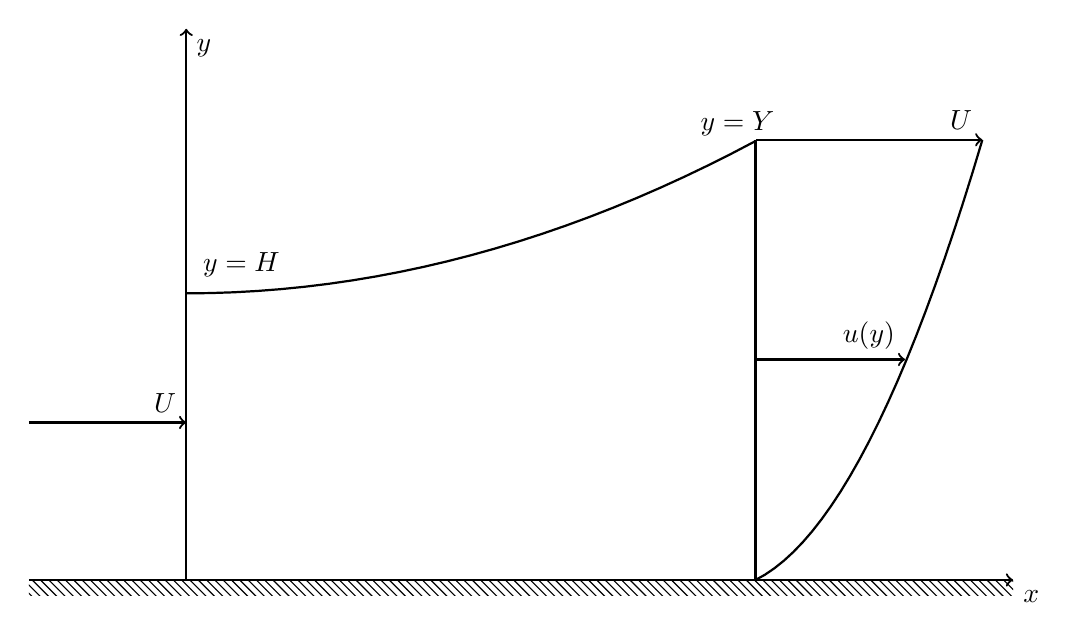
\begin{tikzpicture}
  \draw[thick, ->] (-4,-2) -- (8.5,-2) node[anchor=north west] {$x$};
  \draw[thick, ->] (-2,-2) -- (-2,5) node[anchor=north west] {$y$};

  \draw[thick] (5.23,-2) -- (5.23,3.59);

  \draw (-1.3,2) node {$y=H$};
  \draw (5.0,3.8) node {$y=Y$};



  \draw[thick, ->] (5.23,0.8) -- (7.13,0.8) node[anchor=south east] {$u(y)$};
  \draw[thick, ->] (-4,0) -- (-2,0) node[anchor=south east] {$U$};
  \draw[thick, ->] (5.23, 3.59) -- (8.11, 3.59) node[anchor=south east] {$U$};


  \fill[pattern=north west lines] (-4,-2.2) rectangle ++(12.5,0.2); 


  \begin{scope}[shift={(-2,1.64)}]
  \draw[thick, rotate=0, domain=0:7.23] plot ({\x},{0.037*\x*\x});
  \end{scope}


  \begin{scope}[shift={(5.23,-2)}]
    %\draw[thick, rotate=0, domain=0:2] plot ({\x},{sqrt(1 - \x*\x*0.5)});
    \draw[thick, rotate=0, domain=0:2.88] plot ({\x},{0.5*\x*\x + 0.5*\x});
  \end{scope}

\end{tikzpicture}
\end{document}
